\begin{name}
	{\tenchude}{\tendethi}{LỚP TOÁN THẦY PHÁT}{\thoigian}
\end{name}
\setcounter{ex}{0}\setcounter{bt}{0}
\Opensolutionfile{ans}[ans/ans-2-TT-29-ChuyenVinh-Lan1-23]
\begin{ex}%[Thi thử Chuyên ĐH Vinh Lần 1, 2023]%[Trần Hoà, Ex6-2023]%[2D4Y1-1]
Mô-đun của số phức $z=3-2i$ bằng
\choice
{\True $\sqrt{13}$}
{$-\sqrt{3}$}
{$-2 $}
{$3$} 
\loigiai{
Ta có $|3-2i|=\sqrt{3^2+(-2)^2}=\sqrt{13}$.}
\end{ex}
\begin{ex}%[Thi thử Chuyên ĐH Vinh Lần 1, 2023]%[Trần Hoà, Ex6-2023]%[1D2Y2-1]
Công thức tính đúng của tổ hợp chập $3$ của $10$ là
\choice
{$C_{10}^3=\dfrac{10!}{3!}$}
{$C_{10}^3=\dfrac{10!}{7!}$}
{\True $C_{10}^3=\dfrac{10!}{3!7!}$}
{$C_{10}^3=\dfrac{10!}{3\cdot 7}$}
\loigiai{
Tổ hợp chập $3$ của $10$ là $C_{10}^3=\dfrac{10!}{3!\cdot7!}$.}
\end{ex}

\begin{ex}%[Thi thử Chuyên ĐH Vinh Lần 1, 2023]%[Trần Hoà, Ex6-2023]%[2D1Y2-2]%Câu 3
Cho hàm số $y=f(x)$ có đạo hàm trên $\mathbb{R}$ và có bảng biến thiên như hình vẽ \begin{center}
\begin{tikzpicture}
\tkzTabInit[nocadre=false,lgt=1,espcl=2,deltacl=0.6]
{$x$/.6, $f'(x)$/.6,$f(x)$/3}
{$-\infty$,$1$,$2$,$4$,$+\infty$}
\tkzTabLine{,+,$0$,-,$0$,+,$0$,-,}
\draw
(N13) node[above](A){$-\infty$}
(N22) node[below](B){$8$}
($(N32)!.6!(N33)$) node[below](C){$3$}
($(N42)!0.4!(N43)$) node(D){$5$}
(N53) node[above](E){$-\infty$};
\draw[-stealth] (A)--(B);
\draw[-stealth](B)--(C);
\draw[-stealth](C)--(D);
\draw[-stealth](D)--(E);
;
\end{tikzpicture}
\end{center}
 Giá trị cực tiểu của hàm số đã cho là
\choice
{$8$}
{\True $3$}
{$2$}
{$5$}
\loigiai{
Giá trị cực tiểu của hàm số là $3$.}
\end{ex}

\begin{ex}%[Thi thử Chuyên ĐH Vinh Lần 1, 2023]%[Trần Hoà, Ex6-2023]%[2D1Y1-2]%Câu 4
Cho hàm số $y=f(x)$ có bảng xét dấu của đạo hàm $f'(x)$ trên $\mathbb{R}$ như hình vẽ
\begin{center}
    
\begin{tikzpicture}
\tkzTabInit[nocadre=false,lgt=1.2,espcl=2.5,deltacl=0.6]%[nocadre=true\fasle(không\có) kẻ viền bảng ,
%lgt=1,espcl=2]:Độ rộng cột thứ nhât, các cột tiếp theo
{$x$ /.7,$f'(x)$ /.7}{$-\infty$,$-1$,$+\infty$}
%số dòng của x(1), y'(1), y(2), các giá trị điền ở dòng
\tkzTabLine{,-,$0$,+,}%điền dấu, giá trị y'
\end{tikzpicture}
\end{center}


Hàm số $y=f(x)$ đồng biến trên khoảng
\choice
{$(-\infty;-1)$}
{$\mathbb{R}$}
{\True $(-1;+\infty)$}
{$(-2;+\infty)$}
\loigiai{
Hàm số $y=f(x)$ đồng biến trên khoảng $(-1;+\infty)$.}
\end{ex}

\begin{ex}%[Thi thử Chuyên ĐH Vinh Lần 1, 2023]%[Trần Hoà, Ex6-2023]%[2H2Y1-2]%Câu 5
Cho hình trụ có chu vi của một đường tròn đáy bằng $c$, đường cao bằng $h$. Diện tích xung quanh của hình trụ đã cho bằng
\choice
{\True $c\cdot h$}
{$\dfrac{1}{2}\cdot c\cdot h$}
{$\dfrac{1}{3}\cdot c\cdot h$}
{$2 \cdot  c\cdot h$}
\loigiai{
Chu vi đáy $2\pi r=c\Rightarrow r=\dfrac{c}{2\pi}$.\\
Diện tích xung quanh của hình trụ là $S_\text{xq}=2\pi r h=2\pi\cdot\dfrac{c}{2\pi}\cdot h=c \cdot h$. }
\end{ex}

\begin{ex}%[Thi thử Chuyên ĐH Vinh Lần 1, 2023]%[Trần Hoà, Ex6-2023]%[2H3Y1-1]%Câu 6
Trong KG $Oxyz$, điểm nào sau đây {\bf không} thuộc $(Oxy)$?
\choice
{$Q(1; 1; 0)$}
{$M(1; 0; 0)$}
{$P(0; 1; 0)$}
{\True $N(0; 0; 1)$}
\loigiai{
Phương trình mặt phẳng $(Oxy)$ là $z=0$.\\
Ta thấy điểm $N(0; 0; 1)$ có $z_{N}=1 \neq 0$ nên điểm $N(0; 0; 1)$ không thuộc $(Oxy)$.}
\end{ex}

\begin{ex}%[Thi thử Chuyên ĐH Vinh Lần 1, 2023]%[Trần Hoà, Ex6-2023]%[2D2Y5-1]%Câu 8
Nghiệm của phương trình $4^{5x-1}=16$ là
\choice
{\True $x=\dfrac{3}{5}$}
{$x=1$}
{$x=\dfrac{5}{3}$}
{$x=2$}
\loigiai{
Ta có $4^{5x-1}=16 \Leftrightarrow 4^{5x-1}=4^2\Leftrightarrow 5x-1=2 \Leftrightarrow x=\dfrac{3}{5}$.\\
Nghiệm của phương trình $4^{5x-1}=16$ là $x=\dfrac{3}{5}$.}
\end{ex}

\begin{ex}%[Thi thử Chuyên ĐH Vinh Lần 1, 2023]%[Trần Hoà, Ex6-2023]%[2D1Y5-1]%Câu 9
\immini{Đường cong ở hình bên là đồ thị của một trong bốn hàm số dưới đây. Hàm số đó là
\choice
{$y=x^3+2 x^2+2$}
{$y=-x^3+x^2+2$}
{$y=x^4-2 x^2+2$}
{\True $y=-x^4+2 x^2+2$}}{\begin{tikzpicture}[scale=1, font=\footnotesize, line join=round, line cap=round, >=stealth]
\draw[->] (-2,0)--(0,0) node[below right]{$O$}--(2.2,0) node[below]{$x$};
\draw[->] (0,-.5) --(0,3.5) node[right]{$y$};
\draw [domain=-1.7:1.7, samples=100] %
plot (\x, {-1*(\x)^4+2*(\x)^2+2});
\draw[fill] (0,0) circle (1pt);
%\foreach \x/\g in {-1/150,1/110} 
%\draw[fill] (\x,0) circle(.5pt)node [shift={(\g:.3)}] {$\x$};
%\foreach \y/\g in {-1/180,1/0,2/0} 
%\draw[fill] (0,\y) circle(.5pt)node [shift={(\g:.3)}] {$\y$};
\end{tikzpicture}}
\loigiai{
Đường cong là đồ thị của hàm số có dạng $y=a x^4+b x^2+c$. 
Lại có $\displaystyle\lim\limits_{x \rightarrow+\infty}y=-\infty$ nên $a<0$.\\
Vậy hàm số cần tìm là $y=-x^4+2 x^2+2$.}
\end{ex}

\begin{ex}%[Thi thử Chuyên ĐH Vinh Lần 1, 2023]%[Trần Hoà, Ex6-2023]%[2D2Y4-1]%Câu 10
Tập xác định của hàm số $y=\ln (3-x)$ là
\choice
{$(3;+\infty)$}
{\True $(-\infty; 3)$}
{$(-\infty; 3]$}
{$(0; 3)$}
\loigiai{
Điều kiện $3-x>0 \Leftrightarrow x<3$.\\
Tập xác định của hàm số $y=\ln (3-x)$ là $(-\infty; 3)$.}
\end{ex}

\begin{ex}%[Thi thử Chuyên ĐH Vinh Lần 1, 2023]%[Trần Hoà, Ex6-2023]%[2D2Y4-4]%Câu 11
Giá trị lớn nhất của hàm số $y=\mathrm{e}^x$ trên đoạn $[-1; 1]$ là
\choice
{$1$}
{$0$}
{\True $\mathrm{e}$}
{$\dfrac{1}{\mathrm{e}}$}
\loigiai{
Ta có $y'=\mathrm{e}^x>0, \forall x \Rightarrow \max \limits_{[-1; 1]}y=y(1)=\mathrm{e}$.}
\end{ex}

\begin{ex}%[Thi thử Chuyên ĐH Vinh Lần 1, 2023]%[Trần Hoà, Ex6-2023]%[2D1Y5-4]%Câu 12
Số giao điểm của đồ thị hàm số $y=x^3-3x$ với trục hoành là
\choice
{$2$}
{$0$}
{$1$}
{\True $3$} 
\loigiai{
Ta có $x^3-3x=0 \Leftrightarrow x(x^2-3)=0 \Leftrightarrow\hoac{&x=0\\&x=\sqrt{3}\\&x=-\sqrt{3}.}$\\
Vậy số giao điểm của đồ thị hàm số $y=x^3-3 x$ với trục hoành là $3$.
}
\end{ex}

\begin{ex}%[Thi thử Chuyên ĐH Vinh Lần 1, 2023]%[Trần Hoà, Ex6-2023]%[2D3Y1-1]%Câu 13
Họ các nguyên hàm của hàm số $f(x)=3x^2+x+1$ trên $\mathbb{R}$ là
\choice
{\True $x^3+\dfrac{x^2}{2}+x+C$}
{$x^3+x^2+x+C$}
{$3 x^3+x^2+x+C$}
{$3 x^3+\dfrac{x^2}{2}+x+C$}
\loigiai{
Ta thấy $x^3+\dfrac{x^2}{2}+x+C$ là họ nguyên hàm cùa hàm số $f(x)=3x^2+x+1$ .
}
\end{ex}

\begin{ex}%[Thi thử Chuyên ĐH Vinh Lần 1, 2023]%[Trần Hoà, Ex6-2023]%[2D2Y4-2]%Câu 14
Đạo hàm của hàm số $y=2^{x+1}$ là
\choice
{$y'=2^x\ln 2$}
{$y'=(x+1) 2^x$}
{$y'=\dfrac{2^{x+1}}{\ln 2}$}
{\True $y'=2^{x+1}\ln 2$}
\loigiai{Ta có $y'=2^{x+1}\ln 2$.}
\end{ex}

\begin{ex}%[Thi thử Chuyên ĐH Vinh Lần 1, 2023]%[Trần Hoà, Ex6-2023]%[1D3Y4-3]%Câu 15
Cho dãy $(u_n)$ là một cấp số nhân, biết $u_{1}=3$, $u_2=6$. Khi đó giá trị $u_5$ là
\choice
{$72$ }
{\True $48$}
{$8$}
{$-48$}
\loigiai{
Công bội $q=\dfrac{u_2}{u_{1}}=\dfrac{6}{3}=2$.\\
Vậy $u_5=u_{1}q^4=3\cdot 2^4=48$.}
\end{ex}

\begin{ex}%[Thi thử Chuyên ĐH Vinh Lần 1, 2023]%[Trần Hoà, Ex6-2023]%[2D1Y2-1]%Câu 16
Số điểm cực trị của đồ thị hàm số $y=x^4-2 x^2$ là
\choice
{$1$}
{$2$}
{$0$}
{\True $3$}
\loigiai{
Hàm số $y=x^4-2 x^2$ có dạng $y=ax^4+b x^2+c$ ($a \neq 0$) có $a \cdot  b<0$ nên đồ thị hàm số có $3$ điểm cực trị.}
\end{ex}

\begin{ex}%[Thi thử Chuyên ĐH Vinh Lần 1, 2023]%[Trần Hoà, Ex6-2023]%[2D1Y4-1]%Câu 17
Tiệm cận đứng của đồ thị hàm số $y=\dfrac{2x+3}{x-1}$ là đường thẳng
\choice
{$x=-\dfrac{3}{2}$}
{$y=1$}
{\True $x=1$}
{$y=2$}
\loigiai{
Ta có $\lim\limits_{x\to 1^+}\dfrac{2x+3}{x-1}=+\infty$.\\
Vậy tiệm cận đứng của đồ thị hàm số $y=\dfrac{2x+3}{x-1}$ là đường thẳng $x=1$.}
\end{ex}

\begin{ex}%[Thi thử Chuyên ĐH Vinh Lần 1, 2023]%[Trần Hoà, Ex6-2023]%[2H2Y2-1]%Câu 18
Diện tích mặt cầu có đường kính bằng $d$ được tính theo công thức
\choice
{\True $\pi d^2$}
{$4 \pi d^2$}
{$2 \pi d^2$}
{$\dfrac{1}{2}\pi d^2$}
\loigiai{
Mặt cầu có đường kính bằng $d$ có bán kính $R=\dfrac{d}{2}$ có diện tích là $S=4\pi R^2=\pi d^2$}
\end{ex}

\begin{ex}%[Thi thử Chuyên ĐH Vinh Lần 1, 2023]%[Trần Hoà, Ex6-2023]%[2D4Y2-2]%Câu 19
Phần ảo của số phức $z=(1+i)(2-i)$ là
\choice
{$-1$}
{\True $1$}
{$2$}
{$0$}
\loigiai{Ta có $z=(1+i)(2-i)=3+i$.\\
Vậy phần ảo của số phức $z=(1+i)(2-i)$ là $1$.}
\end{ex}

\begin{ex}%[Thi thử Chuyên ĐH Vinh Lần 1, 2023]%[Trần Hoà, Ex6-2023]%[2H1Y3-2]
Tính thể tích khối chóp có đường cao bằng $3$, diện tích đáy bằng $4$.
\choice
{$12$}
{\True $4$}
{$24$}
{$6$}
\loigiai{
Ta có $V=\dfrac{1}{3}\cdot3\cdot 4=4$.
}
\end{ex}

\begin{ex}%[Thi thử Chuyên ĐH Vinh Lần 1, 2023]%[Trần Hoà, Ex6-2023]%[2H3B2-7]%Câu 7
Trong không gian $O x y z$, cho mặt phẳng $(\alpha)\colon x+y+2 z-1=0$. Mặt phẳng $(\alpha)$ song song với mặt phẳng nào sau đây?
\choice
{\True $(Q)\colon 3x+3y+6z-1=0$}
{$(P)\colon 2x+2y+4z-2=0$}
{$(R)\colon x+y-z-1=0$}
{$(S)\colon-x-y-2z+1=0$}
\loigiai{
Mặt phẳng $(\alpha)$ song song với mặt phẳng $(Q)\colon 3x+3y+6z-1=0$ vì $\dfrac{1}{3}=\dfrac{1}{3}=\dfrac{2}{6}\neq \dfrac{-1}{-1}$.}
\end{ex}

\begin{ex}%[Thi thử Chuyên ĐH Vinh Lần 1, 2023]%[Trần Hoà, Ex6-2023]%[2D2B1-2]
Rút gọn biểu thức $P=a^\frac{3}{2}\cdot\sqrt[3]{a}$ với $a>0$ ta được
\choice
{\True $P=a^{\frac{11}{6}}$}
{$P=a^{\frac{9}{2}}$}
{$P=a^{\frac{1}{2}}$}
{$P=a^{\frac{7}{6}}$}
\loigiai{
Ta có $P=a^{\frac{3}{2}}\cdot a^{\frac{1}{3}}=a^{\frac{11}{6}}$.
}
\end{ex}

\begin{ex}%[Thi thử Chuyên ĐH Vinh Lần 1, 2023]%[Trần Hoà, Ex6-2023]%[2H3B3-2]%Câu 20
Trong KG $Oxyz$, cho đường thẳng $\Delta\colon \dfrac{x-1}{3}=\dfrac{y-2}{2}=\dfrac{z-3}{1}$. Phương trình nào sau đây là PTTS của $\Delta$
\choice
{\True $\heva{&x=1+3t\\&y=2+2t\\&z=3+t}$}
{$\heva{&x=-1+3t\\&y=2+2t\\&z=-3+t}$}
{$\heva{&x=3+t\\&y=2+2t\\&z=1+3t}$}
{$\heva{&x=1+t\\&y=2+2t\\&z=3+3t}$}
\loigiai{Đường thẳng $\Delta$ đi qua điểm $M(1;2;3)$ nhận $\overrightarrow{u}=(3;2;1)$ làm véc-tơ chỉ phương nên có PTTS là  $\heva{&x=1+3t\\&y=2+2t\\&z=3+t.}$}
\end{ex}

\begin{ex}%[Thi thử Chuyên ĐH Vinh Lần 1, 2023]%[Trần Hoà, Ex6-2023]%[2D3B2-1]%Câu 21
Cho $f(x)$ liên tục trên $\mathbb{R}$ thỏa mãn $\displaystyle\int\limits_{-1}^1f(x) \mathrm{\,d}x=2, \displaystyle\int\limits_{-1}^0f(x) \mathrm{\,d}x=5$. Khi đó giá trị $\displaystyle\int\limits_0^1(2 f(x)+1) \mathrm{\,d}x$ bằng
\choice
{$-6$}
{$6$}
{\True $-5$}
{$7$}
\loigiai{
Ta có	{\allowdisplaybreaks
		\begin{eqnarray*}
	&&\displaystyle\int\limits_{-1}^1f(x) \mathrm{\,d}x=\displaystyle\int\limits_{-1}^0f(x) \mathrm{\,d}x+\displaystyle\int\limits_0^1 f(x) \mathrm{\,d}x\\
	&\Rightarrow&
	 \displaystyle\int\limits_0^1f(x) \mathrm{\,d}x=\displaystyle\int\limits_{-1}^1 f(x) \mathrm{\,d}x-\displaystyle\int\limits_{-1}^0 f(x) \mathrm{\,d}x=2-5=-3.
		\end{eqnarray*}
Vậy $\displaystyle\int\limits_0^1 (2f(x)+1) \mathrm{\,d}x=\displaystyle\int\limits_0^1 2 f(x) \mathrm{\,d}x+\displaystyle\int\limits_0^1 1\mathrm{\,d}x=2 \displaystyle\int\limits_0^1 f(x) \mathrm{\,d}x+1=-5$.	}	
}
\end{ex}

\begin{ex}%[Thi thử Chuyên ĐH Vinh Lần 1, 2023]%[Trần Hoà, Ex6-2023]%[1H3B3-3]%Câu 22
Cho hình lập phương $ABCD.A'B'C'D'$. Góc giữa $BC'$ và $(A'B'C'D')$ là
\choice
{\True $45^{\circ}$}
{$30^{\circ}$}
{$60^{\circ}$}
{$90^{\circ}$}
\loigiai{
\immini{$(B C',(A'B'C'D'))=(B C', B'C')=\widehat{B C'B'}=45^\circ$ vì tam giác $BC'B'$ vuông cân tại $B'$.}{\begin{tikzpicture}[scale=1,font=\footnotesize,line join = round, line cap = round, >= stealth]
\coordinate (A) at (0,0);
\def\x{3}
\def\y{2}
\def\z{3}
\def\g{30}% goc hbh đáy
\def\n{90} %goc nghiêng
\coordinate (B) at ($(A)+(\x,0)$);
\coordinate (C) at ($(B)+(\g:\y)$);
\coordinate (D) at ($(A)+(C)-(B)$);
\coordinate (A') at ($(A)+(\n:\z)$);
\coordinate (B') at ($(B)+(\n:\z)$);
\coordinate (C') at ($(C)+(\n:\z)$);
\coordinate (D') at ($(D)+(\n:\z)$);
\draw (A)--(B)--(B')--(A')--cycle;
\draw (A')--(D')--(C')--(B') (B)--(C)--(C') (B)--(C');
\draw[dashed] (A)--(D)--(D') (D)--(C);
\foreach \p/\g in {A/-90,B/-90,C/-45,D/-90,A'/180,B'/90,C'/90,D'/90} \draw[] (\p) circle(.5pt) node [shift={(\g:.3)}] {$\p$};
\end{tikzpicture}
}
 }
\end{ex}

\begin{ex}%[Thi thử Chuyên ĐH Vinh Lần 1, 2023]%[Trần Hoà, Ex6-2023]%[2D1B5-3]%Câu 23
\immini{Cho hàm số bậc ba $y=f(x)$ có đồ thị như hình vẽ, phương trình $f(x^2)=1$ có bao nhiêu nghiệm?
\choice
{5}
{\True 3}
{2}
{6}}{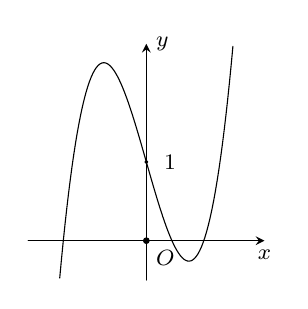
\begin{tikzpicture}[scale=1, font=\footnotesize, line join=round, line cap=round, >=stealth]
\draw[->] (-1.5,0)--(0,0) node[below right]{$O$}--(1.5,0) node[below]{$x$};
\draw[->] (0,-.5) --(0,2.5) node[right]{$y$};
\draw [domain=-1.1:1.1, samples=100] %
plot (\x, {4*(\x)^3-3.5*(\x)+1});
\draw[fill] (0,0) circle (1pt);
%\foreach \x/\g in {-1/150,1/110} 
\foreach \y/\g in {1/0} 
\draw[fill] (0,\y) circle(.5pt)node [shift={(\g:.3)}] {$\y$};
\end{tikzpicture}}
\loigiai{
\immini{Từ đồ thị hàm số ta thấy đường thẳng $y=1$ cắt đồ thị hàm số $y=f(x)$ tại 3 điểm có hoành độ là $a$, $0$, $b$ ($a<0<b$).\\
Suy ra $f(x^2)=1 \Leftrightarrow\hoac{&x^2=a\quad(1)\\&x^2=0\quad(2)\\&x^2=b\quad(3).}$\\
Số nghiệm của phương trình $(1),(2),(3)$ lần lượt là $0,1,2$.\\
Vậy phương trình $f(x^2)=1$ có $3$ nghiệm.}{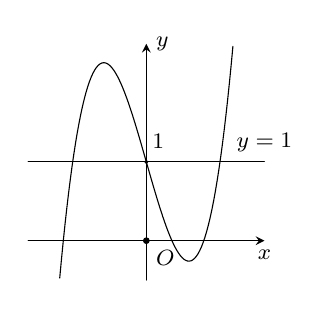
\begin{tikzpicture}[scale=1, font=\footnotesize, line join=round, line cap=round, >=stealth]
\draw[->] (-1.5,0)--(0,0) node[below right]{$O$}--(1.5,0) node[below]{$x$};
\draw[->] (0,-.5) --(0,2.5) node[right]{$y$};
\draw [domain=-1.1:1.1, samples=100] %
plot (\x, {4*(\x)^3-3.5*(\x)+1});
\draw[fill] (0,0) circle (1pt);
%\foreach \x/\g in {-1/150,1/110} 
\foreach \y/\g in {1/60} 
\draw[fill] (0,\y) circle(.5pt)node [shift={(\g:.3)}] {$\y$};
\draw (-1.5,1)--(1.5,1)node[above]{$y=1$};
\end{tikzpicture}}
}
\end{ex}

\begin{ex}%[Thi thử Chuyên ĐH Vinh Lần 1, 2023]%[Trần Hoà, Ex6-2023]%[2D3B3-1]
Diện tích hình phẳng giới hạn bởi hai đồ thị hàm số $y=x^2-4x+3$  và $y=x-1$ bằng
\choice
{$\dfrac{3}{2}$}
{\True $\dfrac{9}{2}$}
{$1$}
{$-\dfrac{9}{2}$}
\loigiai{
Xét phương trình hoành độ giao điểm
	{\allowdisplaybreaks
		\begin{eqnarray*}
	x^2-4x+3=x-1\Leftrightarrow x^2-5x+4=0\Leftrightarrow\hoac{&x=1\\&x=4.}	
		\end{eqnarray*}
	}	
\noindent Suy ra, diện tích hình phẳng đã cho bằng
{\allowdisplaybreaks
		\begin{eqnarray*}
	\displaystyle\int\limits_{1}^{4} |(x^2-4x+3-(x-1))|\mathrm{\,d}x
	&=&
	\displaystyle\int\limits_{1}^{4}|x^2-5x+4|\mathrm{\,d}x\\
	&=&\displaystyle\int\limits_{1}^{4}(-x^2+5x-4)\mathrm{\,d}x=\dfrac{9}{2}.
		\end{eqnarray*}
	}

}
\end{ex}

\begin{ex}%[Thi thử Chuyên ĐH Vinh Lần 1, 2023]%[Trần Hoà, Ex6-2023]%[2D2B3-2]
Cho $\log_ab=2$, $\log_bc=3$. Khi đó giá trị của biểu thức $\log_c(a^2b)$ là
\choice
{$6$}
{$\dfrac{3}{2}$}
{$\dfrac{1}{6}$}
{\True $\dfrac{2}{3}$}
\loigiai{
Ta có $\log_c(a^2b)=\dfrac{\log_b(a^2b)}{\log_bc}=\dfrac{2\log_ba+1}{\log_bc}=\dfrac{\dfrac{2}{\log_ab}+1}{\log_bc}=\dfrac{2}{3}$.
}
\end{ex}

\begin{ex}%[Thi thử Chuyên ĐH Vinh Lần 1, 2023]%[Trần Hoà, Ex6-2023]%[2D3B1-3]
Cho $F(x)$ là một nguyên hàm của hàm số $f(x)=x\sin x$. Biết $F(0)=1$, giá trị $F\left(\dfrac{\pi}{2}\right)$ bằng
\choice
{$0$}
{\True $2$}
{$1+\dfrac{\pi}{2}$}
{$-1$}
\loigiai{
Đặt $\heva{&u=x\\&\mathrm{\,d}v=\sin x\mathrm{\,d}x}\Rightarrow\heva{&\mathrm{\,d}u=\mathrm{\,d}x\\&v=-\cos x.}$\\
$F(x)=-x\cos x+\displaystyle\int \cos x\mathrm{\,d}x=-x\cos x+\sin x+C$.
Mà $F(0)=1$ nên $C=1$, suy ra $F\left(\dfrac{\pi}{2}\right)=2$.
}
\end{ex}

\begin{ex}%[Thi thử Chuyên ĐH Vinh Lần 1, 2023]%[Trần Hoà, Ex6-2023]%[2D4B4-2]
Cho phương trình bậc hai $z^2+bz+c=0$, trong đó $b$, $c$ là các số thực. Với giá trị nào của $b$ thì phương trình đã cho nhận số phức $3+2i$ làm nghiệm?
\choice
{$-5$}
{$6$}
{\True $-6$}
{$5$}
\loigiai{
Phương trình có một nghiệm $z_1=3+2i$ nên nghiệm còn lại là $z_2=3-2i$.\\
Theo định lí Vi-ét $z_1+z_2=-b\Rightarrow b=-6$.
}
\end{ex}

\begin{ex}%[Thi thử Chuyên ĐH Vinh Lần 1, 2023]%[Trần Hoà, Ex6-2023]%[2H3B3-2]
Trong KG $Oxyz$, cho mặt cầu $(S)\colon (x-1)^2+(y-1)^2+(z-2)^2=9$. Viết phương trình mặt phẳng $(\alpha)$ tiếp xúc với $(S)$ tại điểm $M(0;3;0)$.
\choice
{$x-2y+2z-12=0$}
{$x+4y+2z-12=0$}
{\True $x-2y+2z+6=0$}
{$x+2y+2z-6=0$}
\loigiai{
Mặt cầu $(S)$ có tâm $I(1;1;2)$ và bán kính $R=3$.\\
Phương trình mặt phẳng $(\alpha)$ qua điểm $M(0;3;0)$ có véc-tơ pháp  tuyến $\overrightarrow{MI}=(1;-2;2)$ là 
$$1(x-0)-2(y-3)+2(z-0)=0\Leftrightarrow x-2y+2z+6=0.$$
}
\end{ex}

\begin{ex}%[Thi thử Chuyên ĐH Vinh Lần 1, 2023]%[Trần Hoà, Ex6-2023]%[2H1B3-2]
Cho hình lăng trụ đứng $ABC.A'B'C'$ có đáy $ABC$ là tam giác vuông tại $B$. Biết rằng $AB=AA'=a$, $AC=a\sqrt{3}$. Tính thể tích khối lăng trụ $ABC.A'B'C'$.
\choice
{\True $\dfrac{a^3\sqrt{2}}{2}$}
{$\dfrac{a^3\sqrt{2}}{6}$}
{$\dfrac{a^3\sqrt{3}}{2}$}
{$\dfrac{a^3\sqrt{3}}{6}$}
\loigiai{
\immini{Ta có $BC=\sqrt{AC^2-AB^2}=a\sqrt{2}$.\\
Diện tích tam giác $ABC$ là $S_{ABC}=\dfrac{1}{2}BA\cdot BC=\dfrac{a^2\sqrt{2}}{2}$.\\
Thể tích khối lăng trụ là $V=AA'\cdot S_{ABC}=\dfrac{a^3\sqrt{2}}{2}$.}{
\begin{tikzpicture}[scale=1,font=\footnotesize,line join = round, line cap = round, >= stealth]
\coordinate (A) at (0,0);
\def\x{3}
\def\y{2}
\def\z{3}
\def\g{-60}% goc  đáy
\def\n{90} %goc nghiêng
\coordinate (B) at ($(A)+(\x,0)$);
\coordinate (C) at ($(A)+(\g:\y)$);
\coordinate (A') at ($(A)+(\n:\z)$);
\coordinate (B') at ($(B)+(\n:\z)$);
\coordinate (C') at ($(C)+(\n:\z)$);
\draw (A)--(C)--(C')--(A')--cycle;
\draw (A')--(B')--(C')
      (B')--(B)--(C)--(C');
\draw[dashed] (A)--(B);
\tkzMarkRightAngle(A,B,C)
\foreach \p/\g in {A/-120,B/-90,C/-45,A'/180,B'/90,C'/70} \draw[] (\p) circle(.5pt) node [shift={(\g:.3)}] {$\p$};
\end{tikzpicture}
}
}
\end{ex}

\begin{ex}%[Thi thử Chuyên ĐH Vinh Lần 1, 2023]%[Trần Hoà, Ex6-2023]%[2H3B3-2]
Trong KG $Oxyz$, đường thẳng $\Delta$ đi qua điểm $M(1;2;-3)$ và vuông góc với mặt phẳng $(\alpha)\colon 3x+2y+1=0$ có phương trình là
\choice
{$\heva{&x=1+3t\\&y=2+2t\\&z=-3+t}$}
{\True $\heva{&x=1+3t\\&y=2+2t\\&z=-3}$}
{$\heva{&x=-1+3t\\&y=-2+2t\\&z=3}$}
{$\heva{&x=-1+3t\\&y=-2+2t\\&z=3+t}$}
\loigiai{
Do $\Delta \perp (\alpha)$ nên nhận $\overrightarrow{n}=(3;2;0)$ làm véc-tơ chỉ phương.\\
PTĐT $\Delta$ là $\heva{&x=1+3t\\&y=2+2t\\&z=-3.} $
}
\end{ex}

\begin{ex}%[Thi thử Chuyên ĐH Vinh Lần 1, 2023]%[Trần Hoà, Ex6-2023]%[2D1B5-3]
Cho hàm số $y=f(x)$ có đạo hàm trên $\mathbb{R}$ và có bảng biến thiên như hình vẽ
\begin{center}
    \begin{tikzpicture}
\tkzTabInit[nocadre=false,lgt=1.2,espcl=2,deltacl=0.6]
{$x$/.6, $f'(x)$/.6,$f(x)$/3}
{$-\infty$,$1$,$3$,$+\infty$}
\tkzTabLine{,-,$0$,+,$0$,-,}
\draw
(N12) node[below](A){$+\infty$}
($(N22)!0.8!(N23)$) node(B){$0$}
($(N32)!.3!(N33)$) node[below](C){$7$}
(N43) node(D)[above]{$-\infty$}
;
\draw[-stealth] (A)--(B);
\draw[-stealth](B)--(C);
\draw[-stealth](C)--(D);
\end{tikzpicture}
\end{center}
Số nghiệm của phương trình $2|f(x)|-3=0$ là
\choice
{$6$}
{$3$}
{\True $4$}
{$5$}
\loigiai{
Ta có $2|f(x)|-3=0\Leftrightarrow |f(x)|=\dfrac{3}{2}\Leftrightarrow\hoac{&f(x)=\dfrac{3}{2}\\&f(x)=-\dfrac{3}{2}.} $\\
Từ bảng biến thiên ta thấy
\begin{center}
    \begin{tikzpicture}
\tkzTabInit[nocadre=false,lgt=1.2,espcl=2,deltacl=0.6]
{$x$/.6, $f'(x)$/.6,$f(x)$/3}
{$-\infty$,$1$,$3$,$+\infty$}
\tkzTabLine{,-,$0$,+,$0$,-,}
\draw
(N12) node[below](A){$+\infty$}
($(N22)!0.81!(N23)$) node[above](B){$0$}
($(N32)!.3!(N33)$) node[](C){$7$}
(N43) node(D)[above]{$-\infty$}
;
\draw[-stealth] (A)--(B);
\draw[-stealth](B)--(C);
\draw[-stealth](C)--(D);
\draw[blue] (1.3,-2.8)--(7.2,-2.8)node[above]{$y=\tfrac{3}{2}$} ;
\draw[red] (1.3,-3.5)--(7.6,-3.5)node[above]{$y=-\tfrac{3}{2}$};
\end{tikzpicture}
\end{center}
Đường thẳng $y=\dfrac{3}{2}$ cắt đồ thị tại ba điểm phân biệt và đường thẳng $y=-\dfrac{3}{2}$ cắt đồ thị tại một điểm.\\ Vậy phương trình đã cho có $4$ nghiệm.
}
\end{ex}

\begin{ex}%[Thi thử Chuyên ĐH Vinh Lần 1, 2023]%[Trần Hoà, Ex6-2023]%[2H2B1-1]
Cho hình nón có đường sinh bằng $2$, góc ở đỉnh bằng $120^\circ$. Thể tích của khối nón đó bằng
\choice
{$\sqrt{3}\pi$}
{$\dfrac{\sqrt{3}\pi}{3}$}
{$\pi$}
{\True $\pi$}
\loigiai{
\immini{Vì góc ở đỉnh bằng $120^\circ$ nên $\widehat{HSA}=60^\circ$.\\ Trong tam giác vuông $HAS$ ta có\\
$r=AH=l\sin60^\circ =\sqrt{3}$, $h=SH=l\cos60^\circ =1$.\\
Thể tích của hình nón là $V=\dfrac{1}{3}\pi r^2h=\dfrac{1}{3}\pi\cdot 3\cdot 1=\pi$. }{\begin{tikzpicture}[scale=.7, font=\footnotesize, line join=round, line cap=round]
\def\r{3} \def\s{0.2} \def\h{5}
\coordinate (A) at (-\r,0);
\coordinate (B) at (\r,0);
\coordinate (S) at (0,\h);
\coordinate (H) at ($(A)!.5!(B)$);
\begin {scope}[yscale=\s ] 
%Cung tron
\draw[dashed] (B) arc (0:180:\r);
\draw[] (B) arc (0:-180:\r);
\end {scope}
\draw (A)--(S)--(B); 
\draw[dashed]
(S)--(H) (A)--(B);
\foreach \p/\g in {S/90,A/180,B/0,H/45} \draw[fill] (\p) circle(.5pt)node [shift={(\g:.3)}] {$\p$};
\end {tikzpicture}}
}
\end{ex}

\begin{ex}%[Thi thử Chuyên ĐH Vinh Lần 1, 2023]%[Trần Hoà, Ex6-2023]%[2H2B1-4]
\immini{Cần bao nhiêu thuỷ tinh để làm một chiếc cốc hình trụ có chiều cao bằng $12$ cm, đường kính đáy bằng $9{,}6$ cm (tính từ mép ngoài cốc), đáy cốc dày $1{,}8$ cm, thành xung quanh cốc dày $0{,}24$ cm (tính gần đúng đến hai chữ số thập phân)?
\choice
{$64{,}39$ cm$^3$}
{\True $202{,}27$ cm$^3$}
{$212{,}31$ cm$^3$}
{$666{,}97$ cm$^3$}}{\begin{tikzpicture}[scale=.6,font=\footnotesize,line join = round, line cap = round, >= stealth]
%\draw[opacity=0.2] (-3,-2) grid (3,6);
\def \ra {3} \def \rb {1} \def\h{6}
\def \rc{.87*\ra} \def \rd{0.75} 
\draw (-\ra,0) arc (-180:0:{\ra} and {\rb});
\draw[dashed] (-\ra,0) arc (180:0:{\ra} and {\rb});
\draw[shift={(0,\h)}] (-\ra,0)  arc (180:-180:{\ra} and {\rb});
%%
\draw[dashed] (-\rc,0) arc (-180:180:{\rc} and {\rd});
\draw[shift={(0,\h)}] (-\rc,0) arc (-180:180:{\rc} and {\rd});
\draw (-\ra,0)--(-\ra,\h) (\ra,0)--(\ra,\h);
\draw[dashed] (-\rc,0)--(-\rc,\h) (\rc,0)--(\rc,\h);
\draw[shift={(0,-0.8)}] (-\ra,0)  arc (180:360:{\ra} and {\rb});
\draw (-\ra,0)--(-\ra,-0.8) (\ra,0)--(\ra,-0.8);
%Ve đường dóng
\coordinate (A) at (-3,6);
\coordinate (B) at (3,6); \coordinate (b2) at (4,6);
\coordinate (C) at (-3,0); \coordinate (c1) at (-3.5,0); \coordinate (c2) at (-3.5,-1);
\coordinate (D) at (3,0); \coordinate (d1) at ($(3,-1)+(0:1)$);
\coordinate (a1) at ($(-3,6)+(90:1.5)$);
\coordinate (b1) at ($(3,6)+(90:1.5)$);
\draw[<->] (a1)--(b1); \draw[<->] (c1)--(c2); \draw[<->] (d1)--(b2);
\tkzLabelSegment[sloped,pos=0.5](a1,b1){$9{,}6$}
\tkzLabelSegment[sloped,pos=0.5,rotate=180](d1,b2){$12$}
\tkzLabelSegment[sloped,pos=0.5,rotate=180](c1,c2){$1{,}8$}
\draw (A)--(a1) (B)--(b1) (B)--(b2) (C)--(c1) (c2)--($(c2)+(0:.5)$) (d1)--($(d1)+(180:1)$);
%\foreach \p/\g in {A/0,B/0,C/0,D/0} \draw[fill] (\p) circle(.5pt) node [shift={(\g:.3)}] {$\p$};
\end {tikzpicture}

}
\loigiai{
Gọi $V_1$, $V_2$ lần lượt là thể tích của chiếc cốc thuỷ tinh và thể tích của khối lượng chất lỏng mà cốc có thể đựng.\\
Ta có $V_1=12\pi\cdot 4{,}8^2=\dfrac{6912}{25}\pi$ (cm$^3$) và $V_2=(12-1{,}8)\pi\cdot\left(\dfrac{9{,}6-2\cdot 0{,}24}{2}\right)^2\approx 666{,}32$ (cm$^3$).\\
Vậy khối lượng thuỷ tinh cần sử dụng là $\dfrac{6912}{25}\pi- 666{,}32\approx 202{,}27$ (cm$^3$).
}
\end{ex}

\begin{ex}%[Thi thử Chuyên ĐH Vinh Lần 1, 2023]%[Trần Hoà, Ex6-2023]%[2D2B5-6]
Vào cuối năm 2022, báo Rossiyskaya Gazeta dẫn lời Bộ trưởng Tài nguyên Nga cảnh báo nước
này sẽ cạn kiệt dầu mỏ sau $28$ năm nữa nếu sản lượng khai thác hằng năm vẫn giữ như năm 2022.
Bắt đầu từ năm $2023$, nếu nước Nga mỗi năm giảm sản lượng khai thác $2\%$ so với năm trước thì sau bao nhiêu năm nữa nước này cạn kiệt dầu mỏ (chọn phương án có kết quả gần nhất với tính
toán của bạn)?
\choice
{$48$}
{$30$} 
{\True $42$}
{$36$}
\loigiai{
Gọi $S$  là sản lượng dầu mỏ còn lại của Nga trên thực tế tính từ cuối năm $2022$.\\
Gọi $x$  là sản lượng khai khác hằng năm như năm $2022$.\\
Theo đề bài, ta có $S=28x$.\\
Gọi $n$ là số năm khai thác còn lại với sản lượng khai thác thay đổi hằng năm tính từ $2023$.\\
Lượng khai thác mỗi năm tính từ năm $2023$ là $x\cdot\dfrac{(1-2\%)^n-1}{(1-2\%)-1}=\dfrac{0{,}98^n -1}{-0{,}02}x$.\\
Đến khi khai thác hết ta có phương trình 
$$\dfrac{0{,}98^n -1}{-0{,}02}x=28x\Leftrightarrow n=\log_{0{,}98}(1-0{,}02\cdot 28)\approx 40{,}64.$$
}
\end{ex}

\begin{ex}%[Thi thử Chuyên ĐH Vinh Lần 1, 2023]%[Trần Hoà, Ex6-2023]%[2H3B3-2]
Trong KG $Oxyz$, cho mặt phẳng $(\alpha)\colon x+by+cz+d=0$ vuông góc với mặt phẳng $(\beta)\colon x+2y+3z+4=0$ và chứa giao tuyến của hai mặt phẳng $(P)\colon x+3y+z-7=0$, $(Q)\colon x-y+z+1=0$. Khi đó $d$ bằng
\choice
{\True $3$}
{$1$}
{$-3$}
{$-1$}
\loigiai{
Ta có véc-tơ pháp tuyến của $(\beta)$, $(P)$, $(Q)$ lần lượt là $\overrightarrow{n}_1=(1;2;3)$, $\overrightarrow{n}_2=(1;3;1)$, $\overrightarrow{n}_3=(1;-1;1)$.\\
Khi đó $\overrightarrow{n}_{\alpha}=\left[\overrightarrow{n}_1,[\overrightarrow{n}_2,\overrightarrow{n}_3]\right]=(-8;16;-8)=-8(1;-2;1)$.\\
Gọi $A(x;y;z)\in \Delta$, $\Delta$ là giao tuyến của $(P)$ và $(Q)$, khi đó toạ độ điểm $A$ thoả mãn hệ phương trình
$$\heva{&x+3y+z-7=0\\&x-y+z+1=0.}$$
Cho $x=0$, giải hệ ta được $y=2$, $z=1$, khi đó $A(0;2;1)$.\\
Do $(\alpha)$ chứa giao tuyến của $(P)$ và $(Q)$ nên $(\alpha)$ đi qua $A(0;2;1)$.\\
Phương trình $(\alpha)$ là $x-2(y-2)+z-1=0\Leftrightarrow x-2y+z+3=0$. Vậy $d=3$.
}
\end{ex}

\begin{ex}%[Thi thử Chuyên ĐH Vinh Lần 1, 2023]%[Trần Hoà, Ex6-2023]%[1D2K5-4]%Câu 24
Có 6 bạn nam trong đó có Hoàng và 3 bạn nữ xếp ngẫu nhiên thành một hàng ngang. Xác suất để không có hai bạn nữ nào đứng cạnh nhau và Hoàng đứng ở ngoài cùng bằng
\choice
{$\dfrac{10}{21}$}
{$\dfrac{5}{126}$}
{$\dfrac{5}{21}$}
{\True $\dfrac{5}{63}$}
\loigiai{
\begin{itemize}
\item Số cách xếp tùy ý $9$ bạn thành hàng ngang là $9!$ $\Rightarrow n(\Omega)=9!$.
\item Số cách xếp sao cho không có hai bạn nữ nào đứng cạnh nhau và Hoàng đứng ở ngoài cùng
\begin{itemize}
\item Xếp $6$ bạn nam thành một hàng ngang sao cho Hoàng đứng ở ngoài cùng, có $2\cdot 5!$ cách.
\item Xếp 3 bạn nữ vào 6 khoảng trống tạo bởi 6 bạn nam đã được xếp, trừ khoảng trống ngoài cùng bên cạnh Hoàng, có $\mathrm{A}_6^3$ cách.
\end{itemize}
\end{itemize}
Vậy số cách xếp để không có hai bạn nữ nào đứng cạnh nhau và Hoàng đứng ở ngoài cùng bằng: $2\cdot 5 ! \cdot \mathrm{A}_6^3$. Suy ra, xác suất để không có hai bạn nữ nào đứng cạnh nhau và Hoàng đứng ở ngoài cùng bằng $\dfrac{2\cdot 5! \cdot \mathrm{A}_6^3}{n(\Omega)}=\dfrac{2\cdot 5! \cdot  \mathrm{A}_6^3}{9!}=\dfrac{5}{63}$.
}
\end{ex}

\begin{ex}%[Thi thử Chuyên ĐH Vinh Lần 1, 2023]%[Trần Hoà, Ex6-2023]%[1H3K5-3]
Cho hình chóp $S.ABCD$ có đáy hình vuông cạnh $a$, $SAB$ là tam giác đều và nằm trong mặt vuông góc với mặt phẳng đáy. Tính khoảng cách từ $A$ đến $(SCD)$.
\choice
{\True $\dfrac{a\sqrt{21}}{7}$}
{$\dfrac{a\sqrt{2}}{2}$}
{$\dfrac{a\sqrt{3}}{7}$}
{$\dfrac{a\sqrt{2}}{4}$}
\loigiai{
\immini{Gọi $H$ là trung điểm của $AB$, suy ra $SH\perp (ABCD)$.\\
Kẻ $HM\perp CD$ tại $M$.\\
Ta có $\heva{&CD\perp HM\\&CD\perp SH}\Rightarrow CD\perp (SHM)$.\\
Mà $CD\subset (SCD)$ nên $(SHM)\perp (SCD)$ theo giao tuyến $SM$.\\
Trong mặt phẳng $(SHM)$, kẻ $HK\perp SM$ tại $K$. Suy ra $HK \perp (SCD)$.\\
}{\begin{tikzpicture}[scale=1,font=\footnotesize,line join = round, line cap = round, >= stealth]
\coordinate (A) at (0,0);
%\draw[opacity=0.3] (-3,-3) grid (3,3);
\def\x{3.2}
\def\y{1.6}
\def\z{2.7}
\def\g{-130}% goc hbh đáy
\def\n{90} %goc nghiêng
\coordinate (B) at ($(A)+(\g:\y)$);
\coordinate (D) at ($(0:\x)$);
\coordinate (C) at ($(B)+(D)-(A)$);
\coordinate (H) at ($(A)!0.5!(B)$);
\coordinate (S) at ($(H)+(\n:\z)$);
\coordinate (M) at ($(C)!0.5!(D)$);
\coordinate (K) at ($(S)!0.57!(M)$);
\draw (S)--(B)--(C)--cycle;
\draw (S)--(D)--(C) (S)--(M);
\draw[dashed] (S)--(A)--(B) (D)--(A) (A)--(C) (B)--(D);
\draw[dashed] (S)--(H)--(M) (H)--(K);
\foreach \p/\g in {A/40,B/-85,C/-65,D/20,S/90,H/-90,M/-10,K/30} \draw[] (\p) circle(.5pt) node [shift={(\g:.3)}] {$\p$};
\end{tikzpicture}
}
\noindent Vì $AB\parallel (SCD)$ nên $\mathrm{d}(A,(SCD))=\mathrm{d}(H,(SCD))=HK=\dfrac{SH\cdot HM}{\sqrt{SH^2+HM^2}}=\dfrac{a\sqrt{21}}{7}$.
}
\end{ex}

\begin{ex}%[Thi thử Chuyên ĐH Vinh Lần 1, 2023]%[Trần Hoà, Ex6-2023]%[2D1K2-1]
Cho hàm số $y=f(x)$ có đạo hàm trên $\mathbb{R}$ là $f'(x)=x(x-1)^2(x+2)$. Khi đó, hàm số $y=f(-2x)$ đạt cực đại tại
\choice
{$x=-\dfrac{1}{2}$}
{$x=0$}
{\True $x=1$}
{$x=-1$}
\loigiai{
Xét $f'(x)=0\Leftrightarrow x(x-1)^2(x+2)=0\Leftrightarrow\hoac{&x=0\\&x=1\,\text{(bội chẵn)}\\&x=-2.}$\\
Khi đó bảng biến thiên của hàm số $y=f(x)$ như sau
\begin{center}
    
\begin{tikzpicture}
\tkzTabInit[nocadre=false,lgt=1.2,espcl=2,deltacl=0.6]%[nocadre=true\fasle(không\có) kẻ viền bảng ,
%lgt=1,espcl=2]:Độ rộng cột thứ nhât, các cột tiếp theo
{$x$ /.7,$f'(x)$ /.7,$f(x)$ /3}{$-\infty$,$-2$,$0$,$1$,$+\infty$}
%số dòng của x(1), y'(1), y(2), các giá trị điền ở dòng
\tkzTabLine{,+,$0$,-,$0$,+,$0$,+,}%điền dấu, giá trị y'
\tkzTabVar{-/ $-\infty$ ,+/$f(-2)$,-/$f(0)$,R,+/$+\infty$} %-/ là giá trị ở dưới thấp
\end{tikzpicture}
\end{center}
Xét $y=f(-2x)$, ta có $y'=-2f'(-2x)=0\Leftrightarrow\hoac{&-2x=-2\\&-2x=0}\Leftrightarrow\hoac{&x=1\\&x=0.}$\\
Khi đó bảng biến thiên của hàm số $y=f(-2x)$ như sau
\begin{center}
    
\begin{tikzpicture}
\tkzTabInit[nocadre=false,lgt=1,espcl=2,deltacl=0.6]%[nocadre=true\fasle(không\có) kẻ viền bảng ,
%lgt=1,espcl=2]:Độ rộng cột thứ nhât, các cột tiếp theo
{$x$ /.7,$y'$ /.7,$y$ /2}{$-\infty$,$0$,$1$,$+\infty$}
%số dòng của x(1), y'(1), y(2), các giá trị điền ở dòng
\tkzTabLine{,-,$0$,+,$0$,-,}%điền dấu, giá trị y'
\tkzTabVar{+/ $+\infty$ ,-/$y(0)$,+/$y(1)$,-/$-\infty$} %-/ là giá trị ở dưới thấp
\end{tikzpicture}
\end{center}
Vậy hàm số $y=f(-2x)$ đạt cực đại tại $x=1$.
}
\end{ex}

\begin{ex}%[Thi thử Chuyên ĐH Vinh Lần 1, 2023]%[Trần Hoà, Ex6-2023]%[2D1K3-2]
Cho hàm số $y=x^3+mx^2+(2m^2-m+1)x+m^2-3m$. Gọi $S$ là tập hợp tất cả các giá trị thực của tham số $m$ sao cho giá trị lớn nhất của hàm số  trên $(-\infty;0]$ bằng $-2$. Tích các phần tử của $S$ bằng
\choice
{$0$}
{$1$}
{$3$}
{\True $2$}
\loigiai{
Ta có $y'=3x^2+2mx+2m^2-m+1$.\\
Vì $y'$ có $a=3>0$ và $\Delta' = -5m^2+3m-3<0$, $\forall m\in\mathbb{R}$ do đó hàm số đã cho đồng biến trên $\mathbb{R}$, nên $\max\limits_{(-\infty;0]}y=y(0)=m^2-3m$.\\
Theo đề bài ta có $m^2-3m=-2\Leftrightarrow m^2-3m+2=0\Leftrightarrow\hoac{&m=1\\&m=2.}$\\
Do đó $S=\{1;2\}$. Vậy tích các phần tử của $S$ bằng $1\cdot 2 = 2$.
}
\end{ex}

\begin{ex}%[Thi thử Chuyên ĐH Vinh Lần 1, 2023]%[Trần Hoà, Ex6-2023]%[2H1K3-2]
Cho lăng trụ tứ giác đều $ABCD.A'B'C'D'$ có $AA'=1$, tang của góc giữa hai mặt phẳng $(A'BD)$ và $(ABB'A')$ bằng $2$. Tính thể tích của khối lăng trụ $ABCD.A'B'C'D'$.
\choice
{$5$}
{\True $3$}
{$5\sqrt{5}$}
{$3\sqrt{3}$}
\loigiai{
\immini{Gọi $\alpha$ là góc giữa hai mặt phẳng $(A'BD)$ và $(ABB'A')$.\\
Theo bài có $\tan\alpha =2\Rightarrow \sin\alpha =\dfrac{2}{\sqrt{5}}$.\\
Giả sử cạnh đáy của lăng trụ là $x$ ($x>0$).\\
Gọi $I$ là hình chiếu của $D$ trên $A'B$ và $O$ là tâm hình vuông $ABCD$.\\
Ta có $A'D=\sqrt{x^2+1}$, $BD=x\sqrt{2}$, $A'B=\sqrt{x^2+1}$, $A'O=\dfrac{\sqrt{x^2+2}}{\sqrt{2}}$.\\
Ta có $A'O\cdot BD=DI\cdot A'B\Leftrightarrow DI=\dfrac{A'O\cdot BD}{A'B }=\dfrac{\sqrt{x^2+2}\cdot x}{ \sqrt{x^2+1}}$.\\
Dễ thấy $DA\perp (ABB'A')$, $(ABB'A')\cap (A'BD)=A'B$.\\
}{\begin{tikzpicture}[scale=1,font=\footnotesize,line join = round, line cap = round, >= stealth]
\coordinate (A) at (0,0);
\def\x{4}
\def\y{2}
\def\z{3}
\def\g{-120}% goc hbh đáy
\def\n{90} %goc nghiêng
\coordinate (D) at ($(A)+(\x,0)$);
\coordinate (C) at ($(D)+(\g:\y)$);
\coordinate (B) at ($(A)+(C)-(D)$);
\coordinate (A') at ($(A)+(\n:\z)$);
\coordinate (B') at ($(B)+(\n:\z)$);
\coordinate (C') at ($(C)+(\n:\z)$);
\coordinate (D') at ($(D)+(\n:\z)$);

\coordinate (O) at ($(D)!.5!(B)$);
\coordinate (I) at ($(A')!.5!(B)$);
\draw (A')--(D')--(C')--(B')--cycle
(B')--(B)--(C)--(C') 
(C)--(D)--(D')
;
\draw[dashed] (A')--(A)--(B) (A)--(D)
(B)--(A')--(D)--(B) (A)--(C) (D)--(I)
(A')--(O);
\tkzMarkRightAngles(D,O,A' A',I,D)
\foreach \p/\g in {A/-90,B/-90,C/-45,D/-90,A'/180,B'/90,C'/90,D'/90,I/170,O/-90} \draw[] (\p) circle(.5pt) node [shift={(\g:.3)}] {$\p$};
\end{tikzpicture}}
Ta có 	{\allowdisplaybreaks
		\begin{eqnarray*}
	&& \sin\alpha =\dfrac{\mathrm{d}(D,(ABB'A')}{\mathrm{d}(D,A'B)}=\dfrac{DA}{DI}=\dfrac{2}{\sqrt{5}}\\
	&\Leftrightarrow&
	 x\cdot\dfrac{\sqrt{x^2+1}}{\sqrt{x^2+2}\cdot x}=\dfrac{2}{\sqrt{5}}\\
	 &\Leftrightarrow&
	 \dfrac{x^2+1}{x^2+2}=\dfrac{4}{5}\Leftrightarrow x=\sqrt{3}.
	     \end{eqnarray*}
\noindent Vậy $S_{ABCD}=3\Rightarrow V_{ABCD.A'B'C'D'}=3$.	
		
	}
}
\end{ex}

\begin{ex}%[Thi thử Chuyên ĐH Vinh Lần 1, 2023]%[Trần Hoà, Ex6-2023]%[2D3K2-2]
Giả sử hàm số $f(x)$ liên tục trên $\mathbb{R}$, thoả mãn $f(\sin x+1)=\cos x$ với mọi $x\in\mathbb{R}$, khi đó tích phân $\displaystyle\int\limits_1^{\frac{3}{2}}f(x)\mathrm{\,d}x$ bằng
\choice
{$\dfrac{\pi}{12}+\dfrac{\sqrt{3}}{4}$}
{$\dfrac{-\pi}{6}+\dfrac{\sqrt{3}}{4}$}
{$\dfrac{\pi}{12}-\dfrac{\sqrt{3}}{8}$}
{\True $\dfrac{\pi}{12}+\dfrac{\sqrt{3}}{8}$}
\loigiai{
Xét tích phân $I=\displaystyle\int\limits_1^{\frac{3}{2}}f(x)\mathrm{\,d}x$.\\
Đặt $x=\sin t+1\Rightarrow \mathrm{\,d}x=\cos t\mathrm{\,d}t$.\\
Đổi cận $x=1\Rightarrow t=0$, $x=\dfrac{3}{2}\Rightarrow t=\dfrac{\pi}{6}$.\\
Khi đó 
	{\allowdisplaybreaks
		\begin{eqnarray*}
	I&=&\displaystyle\int\limits_0^{\frac{\pi}{6}}f(\sin t+1)\cos t\mathrm{\,d}t
           =\displaystyle\int\limits_0^{\frac{\pi}{6}}\cos t\cdot \cos t \mathrm{\,d}t\\
           &=&\displaystyle\int\limits_0^{\frac{\pi}{6}}\cos^2 t \mathrm{\,d}t
=\displaystyle\int\limits_0^{\frac{\pi}{6}} \left(\dfrac{1}{2}+\dfrac{1}{2}\cos2t\right)\mathrm{\,d}t
=\left.\left(\dfrac{1}{2}t+\dfrac{1}{4}\sin2t\right)\right|_0^{\tfrac{\pi}{6}}=\dfrac{\pi}{12}+\dfrac{\sqrt{3}}{8}.	
		\end{eqnarray*}
	}
}
\end{ex}

\begin{ex}%[Thi thử Chuyên ĐH Vinh Lần 1, 2023]%[Trần Hoà, Ex6-2023]%[2D2K4-4]
Xét các số thực dương $x$, $y$ thoả mãn $\dfrac{1}{2}\log_2\dfrac{x}{4}+\log_2y=\dfrac{4-xy^2}{y^2}$. Khi $x+4y$ đạt giá trị nhỏ nhất, giá trị $\dfrac{x}{y}$ bằng
\choice
{$\dfrac{\sqrt{2}}{2}$}
{$\dfrac{1}{2}$}
{$\sqrt{2}$}
{\True $2$}
\loigiai{
Ta có 
	{\allowdisplaybreaks
		\begin{eqnarray*}
	&& \dfrac{1}{2}\log_2\dfrac{x}{4}+\log_2y=\dfrac{4-xy^2}{y^2}\\
	&\Leftrightarrow&
	\dfrac{1}{2}(\log_2 x-\log_2 4)+\log_2 y=\dfrac{4}{y^2}-x\\
	&\Leftrightarrow&
	\log_2 x- 2+2\log_2 y =\dfrac{8}{y^2}-2x\\
	&\Leftrightarrow&
	\log_2 x+2x = 2-2\log_2 y +\dfrac{8}{y^2}\\
	&\Leftrightarrow&
	\log_2 x +2x =\log_2\dfrac{4}{y^2}+2\left(\dfrac{4}{y^2}\right)\quad(*).
		\end{eqnarray*}
	}
Xét hàm số $f(t)=\log_2 t+2t$ với $t>0$, ta có\\
$f'(t)=\dfrac{1}{t\ln 2} +2>0$ với mọi $t>0$ nên $f(t)$ đồng biến trên khoảng $(0;+\infty)$.\\
Do đó $(*)\Leftrightarrow f(x)=f\left(\dfrac{4}{y^2}\right)\Leftrightarrow x=\dfrac{4}{y^2}$.\\
Khi đó $x+4y=\dfrac{4}{y^2}+2y+2y\ge 3\sqrt[3]{16}$.\\
Dấu \lq\lq =\rq\rq\, xảy ra $\Leftrightarrow\heva{&\dfrac{4}{y^2}=2y\\&x=\dfrac{4}{y^2}}\Leftrightarrow\heva{&y=\sqrt[3]{2}\\&x=\sqrt[3]{4^2}.} $\\
Vậy khi $x+4y$ đạt giá trị nhỏ nhất thì $\dfrac{x}{y}=\dfrac{\sqrt[3]{4^2}}{\sqrt[3]{2}}=2$.	
}
\end{ex}

\begin{ex}%[Thi thử Chuyên ĐH Vinh Lần 1, 2023]%[Trần Hoà, Ex6-2023]%[2D3K3-1]
\immini{Cho hàm số bậc ba $y=f(x)$. Đường thẳng $y=ax+b$ tạo với đường $y=f(x)$ hai miền phẳng có diện tích $S_1$, $S_2$ (hình vẽ). Biết $S_1=\dfrac{5}{12}$ và $\displaystyle\int\limits_0^1(1-2x)f'(3x)\mathrm{\,d}x=-\dfrac{1}{2}$, giá trị của $S_2$ bằng
\choice
{\True $\dfrac{8}{3}$}
{$\dfrac{19}{4}$}
{$\dfrac{13}{3}$}
{$\dfrac{13}{6}$}}{\begin{tikzpicture}[scale=1, font=\footnotesize, line join=round, line cap=round, >=stealth]
\draw[->] (-.5,0)--(0,0) node[below right]{$O$}--(3.5,0) node[below]{$x$};
\draw[->] (0,-3) --(0,1) node[right]{$y$};
\draw [domain=-.2:3.1, samples=100] %
plot (\x, {(20/27)*(\x)^3-(26/9)*(\x)^2+(8/3)*(\x)-2});
\draw [domain=-.3:3.2, samples=100] %
plot (\x, {(2/3)*(\x)-2});
\draw[fill] (0,0) circle (1pt);
\foreach \x/\g in {3/140} 
\draw[fill] (\x,0) circle(.5pt)node [shift={(\g:.3)}] {$\x$};
\foreach \y/\g in {-2/180} 
\draw[fill] (0,\y) circle(.5pt)node [shift={(\g:.3)}] {$\y$};
\fill[pattern=north east lines,pattern color=blue,opacity=0.3](0,-2)--plot[domain=0:3, samples=100](\x, {(20/27)*(\x)^3-(26/9)*(\x)^2+(8/3)*(\x)-2})--cycle;
\draw (0.5,-1.5) node{$S_1$};
\draw (2,-1.8) node{$S_2$};
\end{tikzpicture}}
\loigiai{
	{\allowdisplaybreaks
		\begin{eqnarray*}
	\displaystyle\int\limits_0^1(1-2x)f'(3x)\mathrm{\,d}x
	&=&\displaystyle\int\limits_0^1 (1-2x) \mathrm{\,d}\left[\dfrac{1}{3}f(3x)\right]	
	=\left.\dfrac{1}{3}f(3x)(1-2x)\right|_0^1+\dfrac{2}{3}\displaystyle\int\limits_0^1 f(3x)\mathrm{\,d}x\\	
	&=&\dfrac{-1}{3}f(3)-\dfrac{1}{3}f(0)+\dfrac{2}{9}\displaystyle\int\limits_0^3 f(x) \mathrm{\,d}x	
	=\dfrac{2}{3}+\dfrac{2}{9}\displaystyle\int\limits_0^3 f(x) \mathrm{\,d}x=\dfrac{-1}{2}\\
	&\Leftrightarrow&
	\displaystyle\int\limits_0^3 f(x) \mathrm{\,d}x=\dfrac{-21}{4}.	
		\end{eqnarray*}
	}
Khi đó $S_2=\left|\displaystyle\int\limits_0^3 f(x) \mathrm{\,d}x\right|-(S_{OAB}-S_1)=\dfrac{8}{3}$ với $A(0;-2)$, $B(3;0)$.	
}
\end{ex}

\begin{ex}%[Thi thử Chuyên ĐH Vinh Lần 1, 2023]%[Trần Hoà, Ex6-2023]%[2D4G2-3]
Có bao nhiêu số nguyên $a$ để tồn tại số phức $z$ thoả mãn $|z+\overline{z}|+|z-\overline{z}|=16$ và $|iz-4|=a$?
\choice
{\True $10$}
{$5$}
{$9$}
{$6$}
\loigiai{
Đặt $z=x+yi$, ($x,y\in\mathbb{R}$), suy ra $\overline{z}=x-yi$. Ta có
	{\allowdisplaybreaks
		\begin{eqnarray*}
	&& |z+\overline{z}|+|z-\overline{z}|=16\\
	&\Leftrightarrow&
	2|x|+2|y|=16 \Leftrightarrow
	|x|+|y|=8\\
	&\Leftrightarrow&
	\heva{&x+y=8 &\quad(d_1)\quad\quad\text{khi }x\ge 0,y\ge 0\\
	      &x-y=8 &\quad(d_2)\quad\quad\text{khi }x\ge 0,y<0\\
	      &-x-y=8 &\quad(d_3)\quad\quad\text{khi }x< 0,y< 0\\
	      &-x+y=8 &\quad(d_4)\quad\quad\text{khi }x< 0,y\ge 0. }\quad(1)	
		\end{eqnarray*}}Hay điểm $M(x;y)$ biểu diễn số phức $z$ nằm trên các cạnh của hình vuông $ABCD$ như hình.\\
Lại có $|iz-4|=a\Leftrightarrow \heva{&a\ge 0\\&|-y-4+xi|=a}\Leftrightarrow\heva{&a\ge 0\\& x^2+(y+4)^2=a^2.}\quad(2) $
\begin{itemize}
\item Trường hợp $1$. Nếu $a=0$ thì $\heva{&x=0\\&y=-4}$ không thoả mãn điều kiện $(1)$ nên loại.
\item Trường hợp $2$. Nếu $a>0$ điểm $M(x;y)$ biểu diễn số phức $z$ nằm trên đường tròn tâm $I(0;-4)$ bán kính $a$.
\end{itemize}
Để tồn tại số phức $z$ thoả cả hai điều kiện $(1)$ và $(2)$ thì hình vuông $ABCD$ và đường tròn $(I;a)$ phải có điểm chung	
\begin{center}
    \begin{tikzpicture}[scale=.2,font=\footnotesize,line join = round, line cap = round, >= stealth]
\draw[opacity=0.1] (-15,-18) grid (15,10);		
		\def\a{-15} \def\b{15} \def\c{-18} \def\d{10} \def\v{8}
		\coordinate (O) at (0,0);
		\coordinate (M) at (2,3);
		
		\coordinate (I) at (0,-4);
		\coordinate (A) at (0,\v);
		\coordinate (B) at (\v,0);
		\coordinate (C) at (0,-\v);
		\coordinate (D) at (-\v,0);
		\coordinate (E) at ($(B)!(I)!(C)$); %h là hình chiếu của a lên b-c
		\draw (A)--(B)--(C)--(D)--cycle;
		\draw[->] (\a,0)--(\b,0)node[below]{$x$};
		\draw[->] (0,\c)--(0,\d)node[left]{$y$};
		\foreach \p/\g in {A/60,B/70,C/0,D/120,I/0,O/45} \draw[fill] (\p) circle(.5pt)node [shift={(\g:.3)}] {$\p$};
		\draw (I) let\p1 =($(I)-(E)$) in circle ({veclen(\x1,\y1)}) ;
		\draw (I) circle (12);
		\draw (4,4)node[right]{$d_1$};
		\draw (4,-4)node[below]{$d_2$};
		\draw (-4,-4)node[below]{$d_3$};
		\draw (-4,4)node[left]{$d_4$};
		\draw (8,0)node[below]{$8$};
		\end{tikzpicture}
\end{center}
Do đó $\mathrm{d}(I;d_3)\le a\le IA\Leftrightarrow 2\sqrt{2} \le a \le 12$. Kết hợp với $a\in\mathbb{Z}$, ta có $a\in\{3;4;5;\ldots;12\}$.\\
Vậy có $10$ số nguyên thoả mãn.
}
\end{ex}

\begin{ex}%[Thi thử Chuyên ĐH Vinh Lần 1, 2023]%[Trần Hoà, Ex6-2023]%[2D1G1-3]
Cho hàm số $y=f(x)$ có đạo hàm liên tục trên $\mathbb{R}$ và $g(x)=f'(x^3+2)$ có bảng xét dấu như sau
\begin{center}
    
\begin{tikzpicture}
\tkzTabInit[nocadre=false,lgt=1,espcl=2,deltacl=0.6]
{$x$ /.6,$g(x)$ /.6}{$-\infty$,$-2$,$0$,$2$,$3$,$+\infty$}
\tkzTabLine{,+,$0$,-,$0$,+,$0$,-,$0$,+,}
\end{tikzpicture}
\end{center}
Có bao nhiêu số nguyên $m\in [-2023;2023]$ để hàm số $y=f(x-m)$ đồng biến trên $(-\infty;0)$?
\choice
{$2017$}
{$2020$}
{$2019$}
{\True $2018$}
\loigiai{
Ta có  {\allowdisplaybreaks
		\begin{eqnarray*}
	&&g(x)=0\Leftrightarrow f'(x^3+2)=0\\
	&\Leftrightarrow&
	\hoac{&x=-2\\&x=0\\&x=2\\&x=3}\Rightarrow\hoac{&f'(-6)=0\\&f'(2)=0\\&f'(10)=0\\&f'(29)=0}\\
	&\Rightarrow&
	f'(x)=0\Leftrightarrow \hoac{&x=-6\\&x=2\\&x=10\\&x=29.}	
		\end{eqnarray*}}Xét hàm số $h(x)=f(x-m)\Rightarrow h'(x)=f'(x-m)$.\\
Ta có 	{\allowdisplaybreaks
		\begin{eqnarray*}
	&& h'(x)=0\Leftrightarrow f'(x-m)=0\\
        &\Leftrightarrow&
         \hoac{&x-m=-6\\&x-m=2\\&x-m=10\\&x-m=29}\\
        &\Leftrightarrow&
         \hoac{&x=m-6\\&x=m+2\\&x=m+10\\&x=m+29.}	
		\end{eqnarray*}
	}	
\noindent Ta có bảng xét dấu theo khoảng như sau (với $h'(m)=f'(0)=g(-\sqrt[3]{2})<0$)	
\begin{center}
    
\begin{tikzpicture}
\tkzTabInit[nocadre=false,lgt=4,espcl=2,deltacl=0.6]
{$x$ /.6,$h'(x)=f'(x-m)$ /.6}{$-\infty$,$m-6$,$m+2$,$m+10$,$m+29$,$+\infty$}
\tkzTabLine{,+,$0$,-,$0$,+,$0$,-,$0$,+,}
\end{tikzpicture}
\end{center}
Để hàm số đồng biến trên $(-\infty;0)$ thì $m-6\ge 0\Leftrightarrow m\ge 6$,
suy ra $m\in \{6;7;8;\ldots;2023 \}$.\\
Vậy có $2018$ giá trị nguyên của $m$ thoả mãn.
}
\end{ex}

\begin{ex}%[Thi thử Chuyên ĐH Vinh Lần 1, 2023]%[Trần Hoà, Ex6-2023]%[2D4G5-1]
Xét các số phức $z$, $w$, $u$ thoả mãn $|z|=1$, $|w|=2$, $|u|=3$ và $|z+w-u|=|u+z-w|$. Giá trị lớn nhất của $|z-u|$ bằng
\choice
{$\sqrt{10}$}
{$2\sqrt{3}$}
{\True $\sqrt{14}$}
{$4$}
\loigiai{
Gọi $M$, $N$, $P$ lần lượt là điểm biểu diễn của các số phức $z$, $w$, $u$. Khi đó $OM=1$, $ON=2$, $OP=3$ và $|\overrightarrow{OM}+\overrightarrow{ON}-\overrightarrow{OP}|=|\overrightarrow{OP}+\overrightarrow{OM}-\overrightarrow{ON}|$.\\
Ta có
	{\allowdisplaybreaks
		\begin{eqnarray*}
	&&|\overrightarrow{OM}+\overrightarrow{ON}-\overrightarrow{OP}|=|\overrightarrow{OP}+\overrightarrow{OM}-\overrightarrow{ON}|\\
	&\Leftrightarrow&
	|\overrightarrow{OM}-\overrightarrow{NP}|=|\overrightarrow{OM}+\overrightarrow{NP}|\\
	&\Leftrightarrow&
	OM^2-2\overrightarrow{OM}\cdot\overrightarrow{NP}+NP^2=OM^2+2\overrightarrow{OM}\cdot\overrightarrow{NP}+NP^2\\
	&\Leftrightarrow&
	\overrightarrow{OM}\cdot\overrightarrow{NP}=0\\
	&\Leftrightarrow&
	\overrightarrow{OM}(\overrightarrow{OP}-\overrightarrow{ON})=0\\
	&\Leftrightarrow&
	\overrightarrow{OM}\cdot\overrightarrow{OP}=\overrightarrow{OM}\cdot\overrightarrow{ON}\\
	&\Leftrightarrow&
	OM^2+OP^2-MP^2=OM^2+ON^2-MN^2\\
	&\Leftrightarrow&
	MP^2=MN^2+OP^2-ON^2\le (OM+ON)^2+5\le (OM+ON)^2+5\le 14\\
	&\Rightarrow&
	|z-u|=MP\le \sqrt{14}.
		\end{eqnarray*}}}Đẳng thức xảy ra khi $O$, $M$, $N$ thẳng hàng và $O$ nằm giữa $M$, $N$.
\end{ex}

\begin{ex}%[Thi thử Chuyên ĐH Vinh Lần 1, 2023]%[Trần Hoà, Ex6-2023]%[2D1G2-6]
Cho hai hàm số $f(x)=2x^3-9x^2$ và $g(x)=2x^3-3x^2-12x+m$ ($m$ là tham số). Có bao nhiêu số nguyên $m$ để hàm số $h(x)=f(g(x))$ có đúng $6$ điểm cực trị?
\choice
{$23$}
{$21$}
{\True $6$}
{$4$}
\loigiai{
Ta có $h(x)=f(g(x))\Rightarrow h'(x)=g'(x)\cdot f'(g(x))$. Ta có $h'(x)=0\Leftrightarrow\hoac{&g'(x)=0\\&f'(g(x))=0.}$
\begin{itemize}
\item $g'(x)=0\Leftrightarrow6x^2-6x-12x=0\Leftrightarrow\hoac{&x=-1\\&x=2.}$
\item $f'(x)=6x^2-18x=0\Leftrightarrow\hoac{&x=0\\&x=3.}$
\item $f'(g(x))=0\Leftrightarrow\hoac{&g(x)=0\\&g(x)=3}\Leftrightarrow\hoac{&2x^3-3x^2-12x=-m\\&2x^3-2x^2-12x=-m+3.} \quad(1)$
\end{itemize}
Đặt $k(x)=2x^3-3x^2-12x$, ta có $k'(x)=6x^2-6x-12=0\Leftrightarrow\hoac{&x=-1\\&x=2.}$\\
Ta có bảng biến thiên của hàm số $k(x)$ như sau
\begin{center}
    
\begin{tikzpicture}
\tkzTabInit[nocadre=false,lgt=1.2,espcl=2.5,deltacl=0.6]%[nocadre=true\fasle(không\có) kẻ viền bảng ,
%lgt=1,espcl=2]:Độ rộng cột thứ nhât, các cột tiếp theo
{$x$ /.7,$k'(x)$ /.7,$k(x)$ /2}{$-\infty$,$-1$,$2$,$+\infty$}
%số dòng của x(1), y'(1), y(2), các giá trị điền ở dòng
\tkzTabLine{,+,$0$,-,$0$,+,}%điền dấu, giá trị y'
\tkzTabVar{-/ $-\infty$ ,+/$7$,-/$-20$,+/$+\infty$} %-/ là giá trị ở dưới thấp
\end{tikzpicture}
\end{center}
Để hàm số $h(x)$ có $6$ điểm cực trị thì $(1)$ phải có $4$ nghiệm nên
	{\allowdisplaybreaks
		\begin{eqnarray*}
	&&\hoac{&\heva{&-m+3>7\\&-20<-m\le 7}\\&\heva{&-m\le -20\\&-20<-m+3<7}}\Leftrightarrow\hoac{&-7<m\le -4\\&20\le m<23.}
		\end{eqnarray*}
	}
Vậy có $6$ giá trị nguyên của tham số $m$ thoả mãn yêu cầu bài toán.	
}
\end{ex}
\begin{ex}%[Thi thử Chuyên ĐH Vinh Lần 1, 2023]%[Trần Hoà, Ex6-2023]%[2H3G2-8]
Trong KG $Oxyz$, cho tam giác $ABC$ có $A(3;4;4)$, $B(1;2;3)$, $C(5;0;-1)$. Điểm $M$ thay đổi trong không gian thoả mãn $\widehat{ABM}=\widehat{AMC}=90^\circ$. Mặt phẳng $(\alpha)$ đi qua $B$ và vuông góc với $AC$ cắt $AM$ tại $N$. Khoảng cách từ $N$ đến $(ABC)$ có giá trị lớn nhất bằng
\choice
{$\dfrac{4\sqrt{10}}{5}$}
{\True $\dfrac{3\sqrt{5}}{5}$}
{$\dfrac{2\sqrt{10}}{5}$}
{$\dfrac{6\sqrt{5}}{5}$}
\loigiai{
\immini{Ta có $\overrightarrow{BA}=(2;2;1)$, $\overrightarrow{BC}=(4;-2;-4)\Rightarrow \overrightarrow{BA}\cdot\overrightarrow{BC}=0$ do đó $\triangle ABC$ vuông tại $B$
và $BA=3$, $BC=6$.\\
Từ giả thiết suy ra $\heva{&AB\perp BC\\&AB\perp BM}\Rightarrow AB\perp (MBC)$.\\
Gọi $K$ là hình chiếu của $B$ lên $AC$ nên $(BKN)\perp AC$ cố định.\\
Xét $\triangle ABC$  vuông tại $B$ có $BK$ là đường cao nên\\
$\dfrac{1}{BK^2}=\dfrac{1}{BA^2}+\dfrac{1}{BC^2}=\dfrac{1}{3^2}+\dfrac{1}{6^2}=\dfrac{5}{36}\Rightarrow BK=\dfrac{6\sqrt{5}}{5}$.
}{\begin{tikzpicture}[scale=1,font=\footnotesize,line join = round, line cap = round, >= stealth]
%\draw[opacity=0.2] (0,-2) grid (5,5);
\def\x{4} \def\y{1.8} \def\z{3}
\coordinate (B) at (0,0);
\coordinate (C) at (0:\x);
\coordinate (M) at (-55:\y);
\coordinate (A) at (90:\z);
\coordinate (N) at ($(A)!.4!(M)$);
\coordinate (K) at ($(A)!.4!(C)$);
\coordinate (H) at ($(B)!.6!(K)$);
\draw 
(A)--(B)--(M)--(C)--cycle
(A)--(M) (B)--(N)--(K)
;
\draw[dashed]
(C)--(B) (B)--(K) (N)--(H)
;
\foreach \p/\g in {A/90,M/-90,B/180,C/-90,N/60,K/50,H/-80} \draw[fill] (\p) circle(.5pt)node [shift={(\g:.3)}] {$\p$};
\tkzMarkRightAngles(B,M,C B,N,A B,H,N B,K,C)
\end{tikzpicture}}
\noindent Ta có $\heva{&BN\perp AM\\&BN\perp AC}\Rightarrow BN\perp (AMC)\Rightarrow BN\perp NK$.\\
Suy ra $N$ chạy trên đường tròn đường kính $BK=\dfrac{6\sqrt{5}}{5}$.\\
Trong $(BNK)$ kẻ $NH\perp BK\Rightarrow NH\perp (ABC)\Rightarrow NH=\mathrm{d}(N,(ABC))$.\\
Trong tam giác vuông $BNK$ có $NH\le \dfrac{1}{2}BK=\dfrac{3\sqrt{5}}{5}$.\\
Phương trình mặt phẳng $(BCM)$ đi qua $B$ có véc-tơ pháp tuyến $\overrightarrow{BA}=(2;2;1)$ có dạng 
$$2x+2y=z-9=0.$$
Tam giác $BNK$ vuông cân tại $N$ nên $BN=\dfrac{3\sqrt{2}}{\sqrt{5}}$.\\
Xét $\triangle ABM$ vuông tại $B$ có đường cao $BN$ nên
$$\dfrac{1}{BM^2}=\dfrac{1}{BN^2}-\dfrac{1}{BA^2}=\dfrac{5}{18}-\dfrac{1}{3^3}=\dfrac{1}{6}\Rightarrow BM=\sqrt{6}.$$
Gọi $M(a;b;c)$, ta có
	{\allowdisplaybreaks
		\begin{eqnarray*}
	\heva{&BM=\sqrt{6}\\&\overrightarrow{AM}\cdot \overrightarrow{CM}=0\\&M\in (BCM)}
	&\Leftrightarrow&
	\heva{&(a-1)^2+(b-2)^2+(c-3)^2=6\\&(a-3)(a-5)+(b-4)b+(9c-4)(c+1)=0\\&2a+2b+c-9=0}\\
	&\Leftrightarrow&
	\heva{&a^2+b^2+c^2-2a-4b-6c+8=0\\&a^2+b^2+c^2-8a-4b-3c+11=0\\&2a+2b+c-9=0}\\
	&\Leftrightarrow&
	\heva{&(a-1)^2+(b-2)^2+(c-3)^2=6\\&2a-c-1=0\\&2a+2b+c-9=0}\\
	&\Leftrightarrow&
	\heva{&(a-1)^2+(b-2)&2+(c-3)^2=6\\&c=2a-1\\&b=5-2a}\\
	&\Leftrightarrow&
	\heva{&9a^2-30a+20=0\\&c=2a-1\\&b=5-2a}\\
	&\Leftrightarrow&
	\heva{&a=\dfrac{5+\sqrt{5}}{3}\\&b=\dfrac{5+2\sqrt{5}}{3}\\&c=\dfrac{7+2\sqrt{5}}{3}}
	\text{hoặc}
	\heva{&a=\dfrac{5-\sqrt{5}}{3}\\&b=\dfrac{5-2\sqrt{5}}{3}\\&c=\dfrac{7-2\sqrt{5}}{3}.}	
		\end{eqnarray*}
	}
\noindent Vậy khoảng cách từ $N$ đến $(ABC)$ có giá trị lớn nhất bằng $\dfrac{3\sqrt{5}}{5}$ khi $M(a;b;c)$ với $a$, $b$, $c$ như trên.	
}
\end{ex}
\Closesolutionfile{ans}
\begin{indapan}{10}
	{ans/ans-2-TT-29-ChuyenVinh-Lan1-23}
\end{indapan}
